%%%%%%%%%%%%%%%%%%%%%%%%%%%%%%%%%%%%%%%%%%%%%%%%%%%%%%%%%%%%%%%%%%%%%%
% Lớp 11 | Đường thẳng, mặt phẳng. Quan hệ song song trong | Phép chiếu song song
% Dạng 1H4?6-3: Xác định yếu tố song song
% Số câu: 18  (sinh tự động bởi tach_cau.py; từ nay thầy sửa trực tiếp file này)
%%%%%%%%%%%%%%%%%%%%%%%%%%%%%%%%%%%%%%%%%%%%%%%%%%%%%%%%%%%%%%%%%%%%%%

%%%%%%%%%%%%%%%% ĐÚNG/SAI %%%%%%%%%%%%%%%%

% nguồn: Ok_dungsai_lop11_Lan1
\begin{ex}%[1H4H6-3]%[ma:49c643ab]
 Cho hình lập phương $ABCD.A'B'C'D'$. Gọi $M, N, P$ lần lượt là trung điểm $AD, BC$  và $CC'$.
  \choiceTF
  {\True $BD$ song song $B'D'$ và  $DA'$ song song $CB'$}
   {\True$(A'BD)$ song song $(B'CD')$}
  {\True$(MNP)$ song  song $(ABC')$}
  {Thiết diện của  hình lập phương khi cắt bởi mặt phẳng $(MNP)$ là hình thang cân}
 \loigiai{ 
  \begin{center}
   \begin{tikzpicture}[scale=1,font=\footnotesize,line join=round,line cap=round,>=stealth]
      \def\bc{4}
      \def\ba{2}
      \def\h{4}
      \def\gocB{35}
     \coordinate[label=below left:$B$] (B) at (0,0); 
     \coordinate[label=above left:$A$] (A) at  (\gocB:\ba);
     \coordinate[label=below:$C$] (C) at  (\bc,0);
     \coordinate[label=right:$D$] (D)  at ($(C)-(B)+(A)$);
     \coordinate[label=above left:$A'$]  (A') at ($(A)+(90:\h)$);
      \coordinate[label=left:$B'$] (B') at ($(B)-(A)+(A')$);
     \coordinate[label=below right:$C'$]  (C') at ($(C)-(A)+(A')$);
     \coordinate[label=right:$D'$] (D') at  ($(D)-(A)+(A')$);
     \coordinate[label=below:$M$]  (M) at ($(D)!.5!(A)$);
     \coordinate[label=below:$N$]  (N) at ($(B)!.5!(C)$);
      \coordinate[label=left:$P$] (P) at ($(C)!.5!(C')$);
     \coordinate[label=right:$Q$]  (Q) at ($(D)!.5!(D')$);
     \draw (B')--(B)--(C)--(D)--(D')--(A')--(B')--(C')--(D') 
       (C)--(C')
       (N)--(P)--(Q);
     \draw[dashed]  (A')--(A)--(D)
      (A)--(B) 
       (Q)--(M)--(N);
     \foreach \diem in {A,B,C,D,A',B',C',D',M,N,P,Q} \fill (\diem) circle  (1pt);
    \end{tikzpicture}
  \end{center}
  \begin{itemchoice}
   \itemch Đúng. Vì $BDD'B'$  là hình bình hành nên $BD\parallel B'D'$.
   Tương tự, ta có $DA'\parallel  CB'$.
   \itemch Đúng. Vì $BD\parallel  B'D'$ và $DA'\parallel CB'$.
    Suy ra $(A'BD)\parallel (B'CD')$.\\
   \itemch Đúng. Ta có $AB\parallel MN$ và $BC'\parallel NP$ nên $(ABC')\parallel (MNP)$. 
   \itemch Sai. Ta có $MN\subset (MNP)$, $CD\subset( DCC'D')$, $P\in (MNP)\cap (DCC'D')$ và $MN \parallel  DC$ nên giao tuyến của $(MNP)$ và $(DCC'D')$ là đường thẳng qua $P$ và song song $CD$.\\
    Gọi $Q$ là trung điểm $DD'$ thì $PQ$ là giao tuyến của $(MNP)$ và $(DCC'D')$.\\
   Vậy thiết diện là $MNPQ$.\\ 
   Vì $MN\parallel PQ, MN=PQ$ nên thiết diện là hình  hình hành.
  \end{itemchoice}
  }
\end{ex}

% nguồn: Ok_dungsai_lop11_Lan1
\begin{ex}%[1H4H6-3]%[ma:272f8e79]
 Cho hình chóp $S.ABCD$ có đáy  $ABCD$ là một tứ giác lồi. Gọi $M$, $N$, $T$ lần lượt là trung điểm của $SA$, $SC$ và $SD$.
  \choiceTF
   {\True$MN\parallel (ABC)$}
  {\True$(MNT)\parallel  (ABCD)$}
  {Gọi $(\alpha)$ là mặt phẳng đi qua $M$ và song song với $(SBD)$. Thiết  diện của hình chóp với $(\alpha)$ là một tứ giác}
  {Gọi $(\beta)$ là mặt phẳng đi qua $N$ và song song với $(\alpha)$. Gọi $I$ và $J$ lần lượt là giao điểm của  $AC$ với mặt phẳng $(\alpha)$ và $(\beta)$. Khi đó $AC=\dfrac{19}{10}IJ$}
 \loigiai{ 
  \begin{center}
   \begin{tikzpicture}[scale=1,font=\footnotesize,line join=round,line cap=round,>=stealth]
     \def\ad{7} 
      \def\ab{3}
      \def\bc{4}
      \def\as{5}
     \def\gocA{50} 
     \def\gocB{120} 
     \coordinate[label=left:$A$] (A) at (0,0); 
     \coordinate[label=below  left:$B$] (B) at (-\gocA:\ab);
     \coordinate[label=below right:$C$] (C)  at ($(B)+(-5:\bc)$);
     \coordinate[label=right:$D$] (D) at  (\ad,0);
     \coordinate[label=above:$S$] (S) at  (60:\as);
     \coordinate[label=left:$M$] (M) at ($(S)!.5!(A)$); 
     \coordinate[label=right:$N$] (N) at ($(S)!.5!(C)$); 
     \coordinate[label=right:$T$]  (T) at ($(S)!.5!(D)$);
     \coordinate[label=below  right:$K$] (K) at ($(A)!.5!(D)$);
     \coordinate[label=below left:$R$]  (R) at ($(A)!.5!(B)$);
     \coordinate[label=below: $P$] (P) at ($(C)!.5!(B)$); 
     \coordinate[label=right:$Q$] (Q) at  ($(C)!.5!(D)$);
     \path[name path=rk] (R)--(K); 
     \path[name path=ac] (A)--(C); 
     \path[name  path=bd] (B)--(D);
      \path[name path=pq] (P)--(Q);
      \path[name intersections={of= rk and ac,by=I}];
     \path[name intersections={of= bd and  ac,by=O}];
     \path[name intersections={of= pq  and ac,by=J}];
     \coordinate[label=below: $J$] (J)  at (J);
     \coordinate[label=below: $I$] (I) at (I); 
     \coordinate[label=below: $O$] (O) at (O); 
     \draw (A)--(B)--(C)--(D)--(S)--cycle  (B)--(S)--(C)
      (N)--(T) 
      (M)--(R) 
       (P)--(N)--(Q);
      \draw[dashed] (C)--(A)--(D)
       (T)--(M)--(N)
      (P)--(Q) 
      (M)--(K)--(R) 
       (D)--(B)--(K);
     \foreach \diem in {A,B,C,D,I,S,M,N,T,O,K,R,P,J,Q} \fill (\diem) circle (1pt); 
    \end{tikzpicture}
  \end{center}
  \begin{itemchoice}
   \itemch Đúng. Xét tam giác $ASC$ có $MN$ là đường trung bình nên $MN\parallel AC$.\\ $MN$ không nằm  trong $(ABCD)$, $AC\subset (ABCD)$ suy ra $MN\parallel (ABCD)$.
   \itemch Đúng. Theo chứng minh trên ta có $MN\parallel  (ABCD)$, tương tự suy ra $MT \parallel (ABCD)$.\\
   Vậy trong mặt phẳng $(MNT)$ có hai đường thẳng cắt nhau $MN$ và $MT$ cùng song song với $(ABCD)$  nên $(MNT)\parallel (ABCD)$.
   \itemch Sai. Gọi $K, R$ lần lượt là trung điểm của $AD$ và $AB$. Do mặt phẳng $(\alpha)$ đi qua $M$  và song song với $(SBD)$ nên giao tuyến của $(\alpha)$ với $(SAB)$ và $(SAD)$ là $MR$ và $MK$.\\
   Từ đó ta có thiết diện của hình chóp với $(\alpha)$ là tam  giác $MRK$.
   \itemch Sai. Tương tự ta có thiết diện của hình chóp với $(\beta)$ là tam  giác $NPQ$.\\
   Gọi $I, O, J$  lần lượt là giao điểm của $AC$ với $RK, BD, PQ$ ta suy ra $I, J$ chính là giao điểm của $AC$ với $(\alpha)$ và $(\beta)$.\\
   Do $RK$ và $PQ$ là các đường trung bình của tam giác $ABD$ và  tam giác $CBD$ nên ta có $I$ là trung điểm của $AO$, $J$ là trung điểm của $CO$.\\
    Suy ra $AX=XO$, $CY=OY$ và ta có $AC=2IJ$.
  \end{itemchoice}
 } 
\end{ex}

% nguồn: Ok_dungsai_lop11_Lan2
\begin{ex}%[1H4H6-3]%[ma:f373b72d]
	Cho lăng trụ $ABC.A'B'C'$. Gọi $M$, $N$ lần lượt là trung điểm của  $AC$, $AB$. Khi đó
	 \choiceTF
		{\True Hình chiếu song song của  điểm $M$ lên $\left(AA'B'\right)$ theo phương chiếu $CB$ là trung điểm $AB$}
		{Hình chiếu song song của điểm $M$ lên $\left(AA'B'\right)$ theo phương chiếu $CB$ là  điểm $A$}
		{\True Hình chiếu song song của điểm $B'$ lên  $\left(ABC\right)$ theo phương chiếu $C'C$ là điểm $B$}
		{\True Hình chiếu song song của điểm  $N$ lên $\left(A'AC\right)$ theo phương chiếu $BC$ là trung điểm $AC$}
	\loigiai{ 
		\begin{center}
			\begin{tikzpicture}[scale=1,line join =round,line cap =round,font=\footnotesize,declare function={goc=-45; gocx=75; a=4.5; b=0.45*a; h=4;}]
					 \path
						(0,0)  coordinate (A)
						(a,0) coordinate  (C)
						(goc:b)  coordinate (B)
						(gocx:h)  coordinate (A')
						($(gocx:h)+(C)$) coordinate  (C')
						($(gocx:h)+(B)$)  coordinate (B')
						($(A)!.5!(B)$)  coordinate (N)
						($(A)!.5!(C)$) coordinate  (M);
					\draw[dashed]  (A)--(C)
						(M)--(N); 
					\draw (A)--(B)--(C)--(C')--(A')--(B')--(B) 
						(A)--(A') 
						(B')--(C'); 
					\foreach  \x/\goc in {A/-180,B/-90,C/0,A'/-180,B'/-30,C'/0,M/90,N/-120}
					 \fill (\x) circle (1pt) node[shift={(\goc:7pt)}]{$\x$};
				\end{tikzpicture}
		\end{center}
		Ta có $MN$ là đường trung  bình của $\triangle ABC$ nên $MN\parallel CB$.
		\begin{itemchoice}
			 \itemch \textbf{Đúng.}\\
			Vì  $MN\parallel CB$.
			\itemch \textbf{Sai.} 
			\itemch \textbf{Đúng.}\\ 
			Vì $BB'\parallel  CC'$.
			\itemch  \textbf{Đúng.}\\
			Vì  $MN\parallel CB$.
		\end{itemchoice}
	 }
\end{ex}

% nguồn: Ok_dungsai_lop11_Lan2
\begin{ex}%[1H4H6-3]%[ma:d8bf37c0]
	Cho hình lăng trụ $ABC.A'B'C'$, gọi $I$, $I'$ lần lượt là trung điểm của $AB$, $A'B'$.  Cho phép chiếu song song đường thẳng $AI'$, mặt phẳng chiếu $\left(A'B'C'\right)$. Khi đó
	\choiceTF 
		{\True Hình  chiếu của điểm $I$ là điểm $B'$}
		{\True Hình chiếu của điểm $A$ là điểm  $I'$}
		 {Hình chiếu của điểm $A$ là điểm $A'$}
		{Hình chiếu của  điểm $B$ là điểm $B'$}
	 \loigiai{
		\begin{center}
			\begin{tikzpicture}[scale=1,line join =round,line cap =round,font=\footnotesize,declare function={goc=-45; gocx=75; a=4.5; b=0.45*a; h=4;}]
					\path 
						(0,0)  coordinate (A)
						(a,0) coordinate  (C)
						 (goc:b) coordinate (B)
						(gocx:h)  coordinate (A')
						($(gocx:h)+(C)$)  coordinate (C')
						($(gocx:h)+(B)$)  coordinate (B')
						($(A)!.5!(B)$) coordinate  (I)
						 ($(A')!.5!(B')$) coordinate (I');
					\draw[dashed]  (A)--(C);
					\draw  (A)--(B)--(C)--(C')--(A')--(B')--(B)
						 (A)--(A')
						(B')--(C') 
						(I)--(B') 
						(A)--(I'); 
					\foreach \x/\goc  in {A/-180,B/-90,C/0,A'/-180,B'/-30,C'/0,I'/30,I/-120}
					\fill (\x)  circle (1pt) node[shift={(\goc:7pt)}]{$\x$};
				\end{tikzpicture}
		\end{center}
		Ta có $\heva{&AI\parallel B'I' \\  &AI=B'I' }\Rightarrow AIB'I'$ là hình bình hành.
		\begin{itemchoice}
			 \itemch \textbf{Đúng.}\\
			Vì $AI'  \parallel IB'$.
			\itemch  \textbf{Đúng.}\\
			Vì $AI'$ là phương chiếu của phép chiếu song song và $\left(A'B'C'\right)$ là  mặt phẳng chiếu $\left(A'B'C'\right)$.
			\itemch \textbf{Sai.}\\ 
			Vì $AA'$  không song song với $AI'$.
			\itemch  \textbf{Sai.}\\
			Vì $BB'$ không song song với $AI'$. 
		\end{itemchoice}
	 }
\end{ex}

% nguồn: Ok_dungsai_lop11_Lan2
\begin{ex}%[1H4H6-3]%[ma:7c2513ff]
	 Cho hình lăng trụ $ABC.A'B'C'$. Khi đó
	 \choiceTF
		{\True  $AA' \parallel CC'$}
		{$A'$ hình chiếu của $A$ trên mặt  phẳng $\left(A'B'C'\right)$ qua phép chiếu song song theo phương $CC'$}
		{\True Gọi $M$ là một điểm trên đoạn thẳng $AB$. Hình chiếu của $M$ trên mặt phẳng $\left(A'B'C'\right)$ qua phép chiếu song song theo phương $BB'$ là điểm $M'  \in A'B'$}
		{\True Gọi $O$ là tâm của hình bình hành  $BCC'B'$. Ảnh của $O$ qua phép chiếu song song theo phương $AA'$ trên mặt phẳng $\left(A'B'C'\right)$ là trung điểm của $B'C'$}
	 \loigiai{
		\begin{center}
			\begin{tikzpicture}[scale=1,line join =round,line cap =round,font=\footnotesize,declare function={goc=-45; gocx=75; a=4.5; b=0.45*a; h=4;}]
					 \path
						(0,0) coordinate (A) 
						 (a,0) coordinate (C)
						(goc:b) coordinate (B) 
						(gocx:h) coordinate (A') 
						($(gocx:h)+(C)$) coordinate (C') 
						($(gocx:h)+(B)$) coordinate (B') 
						($(A)!.3!(B)$)  coordinate (M)
						($(A')!.3!(B')$)  coordinate (M')
						 ($(C')!.5!(B)$) coordinate (O)
						($(C')!.5!(B')$)  coordinate (I);
					\draw[dashed] (A)--(C); 
					 \draw (A)--(B)--(C)--(C')--(A')--(B')--(B)
						 (A)--(A')
						 (B')--(C')
						(M)--(M') 
						 (B)--(C')
						(B')--(C) 
						 (O)--(I);
					\foreach \x/\goc in  {A/-180,B/-90,C/0,A'/-180,B'/70,C'/0,M'/30,M/-120,O/0,I/90}
					\fill (\x) circle  (1pt) node[shift={(\goc:7pt)}]{$\x$};
				\end{tikzpicture}
		\end{center}
		\begin{itemchoice}
			\itemch \textbf{Đúng.} 
			\itemch \textbf{Sai.}\\ 
			Vì $AA' \parallel CC'$ và $A'$ thuộc $\left(A'B'C'\right)$ nên $A'$ là hình chiếu song song của $A$ trên  mặt phẳng $\left(A'B'C'\right)$ theo phương $CC'$.
			\itemch  \textbf{Đúng.}\\
			Trong mặt phẳng $\left(ABB'A' \right)$, kẻ đường thẳng $MM' \parallel BB'$ với $M' \in A'B'$. Khi đó $M'$ là hình chiếu song song của $M$ trên  mặt phẳng $\left(A'B'C'\right)$ theo phương $BB'$.
			\itemch \textbf{Đúng.}\\ 
			Gọi $I$ là trung điểm của $B'C'$. Vì $OI$ là đường trung bình  của tam giác $BB'C'$ nên $OI\parallel BB' \Rightarrow OI\parallel AA'$ mà $I\in \left(A'B'C'\right)$ nên $I$ là ảnh của $O$ trên mặt phẳng $\left(A'B'C'\right)$ qua phép chiếu song song phương $AA'$.
		\end{itemchoice}
	} 
\end{ex}

% nguồn: Ok_dungsai_lop11_Lan1
\begin{ex}%[1H4V6-3]%[ma:450994df]
 Cho hình chóp $S.ABCD$ có đáy  là hình bình hành, các điểm $M, N, E$ lần lượt là trung điểm của các cạnh $SB, SD$ và $CD$.
 \choiceTF 
   {Giao tuyến của mặt phẳng $(SAB)$ và mặt phẳng $(SCD)$ là đường thẳng qua $S$ và song song $BC$}
  {\True $ME \parallel (SAD)$} 
  {Hai mặt phẳng $(MBD)$ và $(MAC)$  cắt nhau theo giao tuyến $ME$}
  {Thiết diện của hình chóp $S.ABCD$ khi cắt bởi mặt phẳng  $(MNE)$ là một tứ giác lồi}
 \loigiai{ 
  \begin{itemchoice}
   \itemch Sai. Vì $AB \parallel CD$ nên giao tuyến của $(SAB)$ và $(SCD)$ là $Sx  \parallel AB \parallel CD$.
   \itemch Đúng. \begin{center}
   \begin{tikzpicture}[scale=1,font=\footnotesize,line join=round,line cap=round,>=stealth]
      \def\bc{4}
     \def\ba{2} 
      \def\h{4}
     \def\gocB{30} 
     \coordinate[label=below left:$B$] (B) at (0,0); 
     \coordinate[label=above left:$A$] (A) at (\gocB:\ba); 
      \coordinate[label=below:$C$] (C) at (\bc,0);
      \coordinate[label=right:$D$] (D) at ($(C)-(B)+(A)$);
      \coordinate[label=above:$S$] (S) at ($(A)+(0:1)+(90:\h)$);
      \coordinate[label=above:$x$] (x) at ($(B)-(A)+(S)$);
     \coordinate[label=left:$F$] (F)  at ($(B)!.5!(A)$);
     \coordinate[label=below  right:$E$] (E) at ($(C)!.5!(D)$);
     \coordinate[label=left:$M$] (M)  at ($(B)!.5!(S)$);
     \draw (B)--(C)--(D)--(S)--cycle  (S)--(C)
       (x)--(S)--($(A)-(B)+(S)$);
     \draw[dashed]  (A)--(D)
      (S)--(A)--(B) 
      (M)--(E)--(F)--(M); 
     \foreach \diem in {A,B,C,D,S,M,E,F} \fill (\diem) circle  (1pt);
    \end{tikzpicture}
  \end{center}
  Từ $E$ kẻ $EF \parallel  AD$. Ta có $(MFE) \parallel (SAD)$ suy ra $ME \parallel (SAD)$.
  \itemch Sai. Gọi $O$  là tâm hình bình hành $ABCD$ suy ra $\heva{&O\in AC\subset(MAC)\\&O\in BD\subset(MBD)}\Rightarrow MO=(MAC)\cap(MBD)$.
  \itemch Sai.  Dựng thiết diện của hình chóp $S.ABCD$ khi cắt bởi mặt phẳng $(MNE)$. \\
  $(MNE) \cap (SCD)=EN$.  \\
  Kẻ $MI \parallel SC$ suy ra $M, N, E,  I$ đồng phẳng. Ta có
  $(MNE) \cap  (SBC)=SI$.\\
  Trong mặt phẳng $(ABCD)$  có $EI \cap AD=L$.\\
  Trong mặt phẳng $(SAD)$, có $LN  \cap SA=P$.\\
  Suy ra $(MNE)  \cap (SAD)=NP$,
   $(MNE) \cap (SAD)=MP$. \\
  Vậy  thiết diện cần tìm là ngũ giác $MIENP$.
 \end{itemchoice}
} 
\end{ex}

% nguồn: Ok_dungsai_lop11_Lan1
\begin{ex}%[1H4V6-3]%[ma:3cfcf993]
 Cho hình chóp $ S.ABCD $ có  đáy $ ABCD $ là hình bình hành tâm $O$. Gọi $ M $ là trung điểm $ SB $.
  \choiceTF
  {\True Giao tuyến của đường  thẳng $ (MCD) $ và mp$ (SAB) $ là đường thẳng qua $M$ và song song $AB$}
  {Ba giao tuyến của ba mặt  phẳng $(MAB)$, $(MCD)$, $(ABCD)$ đồng quy}
  {\True Giao điểm  $ H $ của đường thẳng $ MD $ và $ (SAC) $ thuộc cạnh $SO$}
  {\True Gọi $ G $ là trọng tâm tam giác $ ACD $, $ L $ là giao điểm của đường thẳng $ AG $ và $ BC $; $ T $ là giao điểm của $ SC $ và $ (AGM) $. Khi đó ba  điểm $ L, M, T $ thẳng hàng}
 \loigiai{ 
  \begin{center}
   \begin{tikzpicture}[scale=1,font=\footnotesize,line join=round,line cap=round,>=stealth]
     \def\bc{4} 
     \def\ba{2.5} 
      \def\h{5}
     \def\gocB{40} 
     \coordinate[label=below left:$B$] (B)  at (0,0);
     \coordinate[label=above  left:$A$] (A) at (\gocB:\ba);
     \coordinate[label=below:$C$]  (C) at (\bc,0);
     \coordinate[label=right:$D$] (D) at  ($(C)-(B)+(A)$);
     \coordinate[label=above:$S$] (S) at  ($(A)+(0:.5)+(90:\h)$);
     \coordinate[label=below:$O$] (O) at ($(A)!.5!(C)$); 
     \coordinate[label=left:$M$] (M) at  ($(S)!.5!(B)$);
     \coordinate[label=above right:$H$]  (H) at ($(S)!2/3!(O)$);
      \coordinate[label=above:$G$] (G) at ($(D)!2/3!(O)$);
     \coordinate[label=below left:$T$]  (T) at ($(S)!2/3!(C)$);
     \coordinate[label=right:$L$] (L) at ($(C)-(B)+(C)$); 
     \coordinate[label=right:$N$] (N)  at ($(S)!.5!(A)$);
     \draw  (B)--(C)--(D)--(S)--cycle (S)--(C)
       ($(C)!.5!(D)$)--(L);
      \draw[dashed] (C)--(A)--(D)--(B)
      (O)--(S)--(A)--(B) 
       (A)--($(C)!.5!(D)$)
      (D)--(M)--(N); 
      \draw[red](L)--(M);
     \foreach \diem in {A,B,C,D,S,G,M,H,T,L,O,N} \fill (\diem)  circle (1pt);
    \end{tikzpicture}
  \end{center}
  \begin{itemchoice}
   \itemch Đúng. Ta có $ M \in (MCD) $ và $ M \in SB \subset (SAB) $ nên $M$ là điểm chung thứ nhất  của hai mặt phẳng $ (MCD) $ và $ (SAB) $. \\
   Mặt khác, $ DC \subset (MDC) $, $ AB  \subset (SAB) $ và $ AB \parallel CD $. \\
   Nên giao tuyến cần tìm là đường thẳng $ d  $ đi qua $ M $ và song song với $ AB $ và cắt $ SA $ tại trung điểm $ N $.
   \itemch Sai. Ta có $(MAB)\cap(MCD)=d$,  $(MAB)\cap(ABCD)=AB$,\\$(MCD)\cap(ABCD)=CD$ nên $d\parallel AB\parallel CD$.
   \itemch Đúng. Trong mp$ (SBD)  $ gọi $H$ là giao điểm của $ SO $ và $ DM $. \\
   Khi đó $ H \in SO \subset (SAC)$, $H \in DM $ nên  $ H = DM \cap (SAC) $.\\
   Suy ra Giao điểm $ H $ của đường thẳng $ MD $ và  $ (SAC) $ thuộc cạnh $SO$
   \itemch Đúng. Ta  có $ L = AG \cap BC \Rightarrow L \in (AGM) \cap (SBC)$. \\
   Ta có $ M \in SB \subset (SBC) \Rightarrow M \in (AGM) \cap  (SBC)$. \\
   Ta có $ N =  SG \cap (AGM) \Rightarrow N \in (AGM) \cap (SBC)$. \\
   Từ đó $ L, M, N $ cùng thuộc giao tuyến của hai mặt phẳng $ (AGM) $ và $ (SBC)  $ nên $ L, M, N $ thẳng hàng.
  \end{itemchoice}
 } 
\end{ex}

% nguồn: Ok_dungsai_lop11_Lan1
\begin{ex}%[1H4V6-3]%[ma:8d1db816]
 Cho hình chóp $ S.ABCD $ có đáy $ ABCD $ là hình thang có đáy lớn là $ AD $. Gọi $ M $,  $ N $ lần lượt là các điểm trên các đoạn thẳng $ SA $ và $ SC $ sao cho $AM = 2MS$; $CN = 2NS$.
 \choiceTF 
  {Đường thẳng $CD$ và mặt phẳng $(SAB)$ không giao  nhau}
  {\True Giao  tuyến của hai mặt phẳng $(SAD)$ và $(SBC)$ song song với $AD$}
  {\True Đường thẳng $MN$  song song mặt phẳng $(BCD)$}
  {\True Thiết diện của hình chóp $S.ABCD$ cắt bởi mặt phẳng $(BMN)$ là một tứ  giác}
  \loigiai{
  \begin{center}
   \begin{tikzpicture}[scale=1,font=\footnotesize,line join=round,line cap=round,>=stealth]
     \def\ac{7} 
      \def\ab{3}
     \def\as{4.5} 
     \def\gocA{50} 
     \coordinate[label=left:$A$] (A) at  (0,0);
      \coordinate[label=right:$D$] (D) at (\ac,0);
     \coordinate[label=below left:$I$] (I) at (-\gocA:\ab); 
      \coordinate[label=above:$S$] (S) at (60:\as);
     \coordinate[label=below  left:$B$] (B) at ($(A)!.7!(I)$);
     \coordinate[label=below  right:$C$] (C) at ($(D)!.7!(I)$);
     \coordinate[label=left:$M$] (M) at ($(A)!2/3!(S)$); 
     \coordinate[label=  right:$N$] (N) at ($(C)!2/3!(S)$);
     \coordinate[label=below left:$B$] (B) at  ($(A)!.7!(I)$);
     \path[name  path=ac] (A)--(C);
     \path[name path=bd]  (B)--(D);
     \path[name intersections={of=  ac and bd,by=O}];
     \coordinate[label=below:$O$] (O) at (O); 
     \path[name path=so] (S)--(O); 
     \path[name  path=mn] (M)--(N);
      \path[name intersections={of= so and mn,by=J}];
     \coordinate[label=below left:$J$] (J) at  (J);
     \path[name  path=bj] (B)--($(J)+.35*(J)-.35*(B)$);
     \path[name  path=sd] (S)--(D);
     \path[name intersections={of= bj and sd,by=K}]; 
      \coordinate[label=above right:$K$] (K) at (K);
     \draw  (A)--(I)--(D)--(S)--cycle (M)--(B)--(N)--(K)
      (B)--(S)--(C)--(B); 
     \draw[dashed] (C)--(A)--(D)--(B) 
       (O)--(S)
       (B)--(K)--(M)--(N);
      \foreach \diem in {A,I,D,S,O,B,C,M,N,J,K}\fill (\diem) circle (1pt);
    \end{tikzpicture}
  \end{center}
  \begin{itemchoice}
   \itemch Sai.  Do $ABCD$ là hình thang có $ AB $ và $ CD $ không song song, gọi $I = AB \cap CD$.\\
   Khi đó, $I \in AB \Rightarrow  I \in (SAB)$ nên I là giao điểm.
   \itemch Đúng. Ta có, $S$ là  điểm chung của hai mặt phẳng.\\
   Trong hai mặt phẳng $ (SAD) $  và $ (SBC) $ lần lượt có $ AD \parallel BC $.\\
   Nên giao tuyến cần tìm là đường thẳng  $ Sx \parallel AD \parallel BC $.
   \itemch Sai. Ta có, $MN$ không thuộc mp$(BCD)$.\\ 
   Mà $\dfrac{SM}{SA}  = \dfrac{1}{3};\dfrac{SN}{SC} = \dfrac{1}{3}$ nên $ MN \parallel AC$.\\
   Vậy $ MN \parallel (ABCD)$ hay  $MN \parallel (BCD)$.
   \itemch Đúng. Gọi $ O=AC \cap BD $. Khi đó, $ SO\cap  MN = J $.\\
    Trong $ (SBD) $ có $ BJ\cap SD $ tại $K$. \\
   Như vậy, thiết diện  cận tìm là tứ giác $ BMKN $.
  \end{itemchoice}
  }
\end{ex}

% nguồn: Ok_dungsai_lop11_Lan1
\begin{ex}%[1H4V6-3]%[ma:ba231c92]
 Cho hình chóp $S.ABC$ có đáy là tam giác vuông cân tại $B$, $AB=BC=a$. Cạnh bên $SA$ vuông góc với mặt phẳng đáy $(ABC)$ và $SA=a$. Gọi $I$ là trung điểm của $AC$  và kẻ $IH \perp SC$.
 \choiceTF 
  {\True  Đường thẳng $SC$ vuông góc với mặt phẳng $(BHI)$}
  {Cô-sin góc tạo bởi hai  đường thẳng $IH$ và $BH$ bằng $\dfrac{\sqrt{3}}{2}$}
  { Độ dài đoạn thẳng  $BH$ bằng $\dfrac{a\sqrt{2}}{2}$}
  {\True Góc giữa hai mặt phẳng  $(SAC)$ và $(SBC)$ bằng $60^\circ$}
 \loigiai{ 
  \begin{enumerate}
   \item \immini{Ta có\\ 
   +) $\heva{&BI\perp AC\\&BI\perp SA\\& AC \cap SA =A}\Rightarrow BI\perp (SAC)\Rightarrow  BI\perp SC$.\\
   +) $\heva{&SC\perp IH\\&SC\perp BI\\& IH \cap BI =I}\Rightarrow SC\perp (BHI)$.}{   \begin{tikzpicture}
  \path 
   (0,0)  coordinate (A)
    (5,0) coordinate (C)
   (2,-2) coordinate  (B)
    (0,5) coordinate (S)
   ($(A)!0.5!(C)$) coordinate (I) 
   ($(S)!3/4!(C)$) coordinate (H) 
    ($(S)!1/2!(C)$) coordinate (K);
  \draw 
    (C)--(S)--(A)--(B)--cycle (A)--(B)
    (S)--(B)
    (B)--(H)
    pic[draw,angle radius=3mm]{right angle=S--H--I}
   pic[draw,angle radius=3mm]{right  angle=A--B--C}
   pic[draw,angle radius=3mm]{right angle=A--K--C} 
    pic[draw,angle radius=3mm]{right angle=S--A--C}
   pic[draw,angle radius=3mm]{right  angle=S--A--B}
    pic[draw,angle radius=3mm]{right angle=A--I--B}
   pic [draw,double,angle  radius=6mm]{angle=I--H--B};
  \draw[dashed]  (A)--(C)
   (B)--(I) 
    (A)--(K)
   (I)--(H); 
   \foreach \x/\g in {A/180,C/0,B/-90,S/90,H/0,K/60,I/120}
  \draw [fill= white] (\x) circle (.05)+(\g:.3)  node{$\x$};
 \end{tikzpicture}
   } 
   \item Áp dụng định lí Py-ta-go  trong $\Delta SAC$: $AC=\sqrt{AB^2+BC^2}=\sqrt{a^2+a^2}=a\sqrt{2}$.\\
   Gọi $K$ là chân đường cao hạ  từ $A$ trong $\Delta SAC$. Trong $\Delta SAC$, ta có:
   \begin{center}
     $\dfrac{1}{AK^2}=\dfrac{1}{SA^2}+\dfrac{1}{AC^2}=\dfrac{1}{a^2}+\dfrac{1}{2a^2}=\dfrac{3}{2a^2}\Rightarrow AK=\dfrac{a\sqrt{6}}{3}$.
   \end{center}
   Ta có $IH$ là đường  trung bình trong $\Delta AKC$ nên $IH=\dfrac{AK}{2}=\dfrac{a\sqrt{6}}{6}$.\\
   Vì $BI$ là đường trung tuyến trong tam  giác vuông $\Delta ABC$ nên $BI=\dfrac{AC}{2}=\dfrac{a\sqrt{2}}{2}$.\\
   Theo chứng minh trên $BI \perp (SAC)\Rightarrow BI \perp  HI$ hay $\Delta IHB$ vuông tại $I$.\\
   Góc giữa hai đường thẳng $IH$ và $BH$ bằng $\widehat{IHB}$. Trong $\Delta  IHB$, có
   \begin{center}
    $\tan\widehat{IHB}=\dfrac{IB}{IH}=\dfrac{\dfrac{a\sqrt{2}}{2}}{\dfrac{a\sqrt{6}}{6}}=\sqrt{3} \Rightarrow \widehat{IHB}=60^\circ$. 
   \end{center}
   Do đó $\cos \widehat{IHB}=\dfrac{1}{2}$. Vậy cosin của góc tạo bởi hai đường thẳng $IH$ và $BH$ bằng  $\dfrac{1}{2}$.
    \item Trong $\Delta IHB$ vuông tại $I$, ta có: $BH=\dfrac{IH}{\cos \widehat{IHB}}=\dfrac{\dfrac{a\sqrt{6}}{6}}{\dfrac{1}{2}}=\dfrac{a\sqrt{6}}{3}$.
   \item Ta có $\heva{&(SAC)\cap (SBC)=SC\\&IH\perp SC\\& BH\perp SC}\Rightarrow  \widehat{((SAC),(SBC))}= \widehat{IHB}=60^\circ$.
  \end{enumerate}
  \begin{itemchoice}
   \itemch  Đúng
   \itemch Sai 
   \itemch  Sai
   \itemch  Đúng
  \end{itemchoice}
 } 
\end{ex}

% nguồn: Ok_dungsai_lop11_Lan2
\begin{ex}%[1H4V6-3]%[ma:59dac6fa]
	Cho hình lăng trụ $ABC.A'B'C'$ gọi $I$ và $I'$ lần lượt là trung  điểm của đoạn $AB$ và $A'B'$. Khi đó
	 \choiceTF
		{\True $AI' \parallel IB'$} 
		{Hình chiếu song song của $I$ trên mặt phẳng $\left(A'B'C'\right)$ phương $A'I$ là điểm $C'$} 
		{\True Trong mặt phẳng $\left(A'B'C'\right)$, vẽ hình bình hành $A'C'MI'$. Suy ra $ACMI'$  là hình bình hành}
		{\True $M$ là hình chiếu song song của  $C$ theo phương $AI'$ trên mặt phẳng $\left(A'B'C'\right)$}
	 \loigiai{
		\begin{center}
			\begin{tikzpicture}[scale=1,line join =round,line cap =round,font=\scriptsize,declare function={goc=-45; gocx=75; a=4.5; b=0.5*a; h=4;}]
					 \path
						(0,0) coordinate (A) 
						(a,0) coordinate  (C)
						 (goc:b) coordinate (B)
						(gocx:h) coordinate  (A')
						($(gocx:h)+(C)$) coordinate (C') 
						($(gocx:h)+(B)$) coordinate  (B')
						($(A)!.5!(B)$)  coordinate (I)
						($(A')!.5!(B')$) coordinate (I') 
						($(C')!.5!(B')$) coordinate  (J)
						($(I')!2!(J)$)  coordinate (M);
					\draw[dashed] (A)--(C)--(C'); 
					\draw  (A)--(B)--(C)
						 (C')--(A')--(B')--(B)
						 (A)--(A')
						 (B')--(C')
						 (A)--(I')--(M)
						(I)--(B') 
						 (C)--(M)--(C');
					\foreach \x/\goc in  {A/-180,B/-90,C/0,A'/-180,B'/-30,C'/90,I'/60,I/-120,J/-90,M/0}
					\fill (\x) circle  (1pt) node[shift={(\goc:7pt)}]{$\x$};
				\end{tikzpicture}
		\end{center}
		\begin{itemchoice}
			\itemch \textbf{Đúng.}\\ 
			Ta có $\heva{&AI\parallel B' I'  \\ &AI=B'I'=\dfrac{AB}{2}}$. Suy ra $AIB'I'$ là hình bình hành. Do đó $AI' \parallel IB'$.
			 \itemch \textbf{Sai.}\\
			Hình chiếu  song song của $I$ trên mặt phẳng $\left(A'B'C' \right)$ theo phương $A'I$ là điểm $B'$.
			\itemch  \textbf{Đúng.}\\
			Trong mặt phẳng $\left(A' B' C' \right)$, vẽ hình bình hành $A'C'MI'$.\\ 
			Vì $\heva{&MI' \parallel A'C',\,MI'=A'C' \\ &A' C' \parallel AC,\,A'C'=AC} \Rightarrow MI' \parallel AC,\,MI'=AC$.\\ 
			Suy  ra $ACMI'$ là hình bình hành.
			\itemch \textbf{Đúng.}\\ 
			Vì vậy $AI' \parallel CM$, mà $M\in \left(A'B'C'\right)$ nên  $M$ chính là hình chiếu song song của $C$ theo phương $AI'$ trên mặt phẳng $\left(A'B'C'\right)$.
		\end{itemchoice}
	 }
\end{ex}


%%%%%%%%%%%%%%%% TRẢ LỜI NGẮN %%%%%%%%%%%%%%%%

% nguồn: Ok_TraLoiNgan_Lop11_Lan1
\begin{ex}%[1H4H6-3]%[ma:620c95e6]
	Cho tứ diện $ABC D$. Điểm $G$ là trọng tâm của tam  giác $ABC$ và $M$ là trung điểm $A B$. Hình chiếu song song của điểm $M$ và $G$ theo phương $C D$ lên mặt phẳng $(ABD)$ là $E$. Khi đó $\overrightarrow{MA}+\overrightarrow{MB}+\overrightarrow{MD}=k\overrightarrow{ME}$. Với điểm $M$ bất kỳ, giá trị của $k$ bằng
	\shortans{3} 
	 \loigiai{
		Vì $M$ thuộc mặt phẳng $(ABD)$ nên hình  chiếu song song của $M$ theo phương $C D$ lên mặt phẳng $(ABD)$ cũng là chính nó.\\
		Gọi $E$ là trọng tâm tam giác $ABD$. Vì $G$, $E$ lần lượt là trọng tâm của tam giác $ABC$, $ABD$ nên $\dfrac{MG}{MC}=\dfrac{ME}{MD}=\dfrac{1}{3} \Rightarrow GE \parallel CD$ (định lí Thalès).\\ 
		Vậy hình chiếu song song của điểm $G$ theo phương  $CD$ lên mặt phẳng $(ABD)$ là trọng tâm $E$ của tam giác $ABD$.\\
	Khi  đó với điểm $M$ bất kỳ, ta có $\overrightarrow{MA}+\overrightarrow{MB}+\overrightarrow{MD}=3\overrightarrow{ME}$ nên giá trị của $k$ bằng $3$.}
\end{ex}

% nguồn: Ok_TraLoiNgan_Lop11_Lan1
\begin{ex}%[1H4V6-3]%[ma:94b0bf71]
	Cho lăng trụ tam giác $ABC.A'B'C'$. Trên tia đối của tia $AC$ lấy điểm $M$  sao cho $AM=AC$. Gọi $E$ là trung điểm của $AB$, $D$ là giao điểm của $BC$ và mặt phẳng $(MB'E)$. Khi đó tỉ số diện tích tam giác $ABC$ và tam giác $BDE$ bằng
	\shortans{6} 
	 \loigiai{
		\begin{center}
			\begin{tikzpicture}[scale=1,line join = round,line cap = round]
					 \def\a{4}
					\def\h{4.5} 
					\path  (0:0) coordinate (A)
						++(0:\a) coordinate  (C)
						++(-135:\a/2) coordinate (B) 
						($(B)!0.5!(C)$)  coordinate (I)
						($(A)!2/3!(I)$) coordinate  (G)
						 ($(G)+(90:\h)$) coordinate (A')
						($(A')+(C)-(A)$)  coordinate (C')
						($(C')+(B)-(C)$) coordinate  (B')
						($(A)!-1!(C)$) coordinate  (M)
						 ($(A)!.5!(B)$) coordinate (E)
						 ($(B)!1/3!(C)$) coordinate (D)
						($(B)!.5!(C)$) coordinate  (F)
						(intersection of B'--M and A--A')  coordinate (K);
					\draw[dashed] (A)--(C) 
						 (E)--(D)
						 (A)--(E)
						 (A)--(K)
						 (A)--(M)
						(E)--(F); 
					\draw (C)--(C') 
						(B)--(B') 
						 (K)--(A')
						 (B')--(D)
						 (M)--(B')--(E)--cycle
						 (E)--(B)--(C)
						 (A')--(B')--(C')--cycle;
					 \foreach \x/\g in {A/120,B/-45,C/0,A'/180,B'/-45,C'/30,M/-150,E/-120,D/-45,F/-10}
					\fill[black] (\x) circle  (1pt)
						($(\g:3mm)+(\x)$) node  {$\x$};
				\end{tikzpicture}
		\end{center}
		 Trong mặt phẳng $(ABC)$, gọi $D=ME\cap BC$.\\
		Khi đó $\heva{&D\in BC\\&D\in ME\subset (MB'E)} \Rightarrow D=BC\cap (MB'E)$.\\ 
		Gọi $F$ là trung  điểm $BC$, ta có $EF$ là đường trung bình $\triangle ABC$.\\
		$\Rightarrow EF=\dfrac{1}{2}AB=\dfrac{1}{4}CM$ và $EF\parallel  CM$.\\
		$\Rightarrow \dfrac{EF}{CM}=\dfrac{DF}{CD}=\dfrac{1}{4}\Rightarrow DF=\dfrac{1}{4}CD\Rightarrow DF=\dfrac{1}{3}FC\Rightarrow BD=\dfrac{1}{3}BC$.\\ 
		Suy ra  $\dfrac{S_{\triangle ABC}}{S_{\triangle BDE}}=\dfrac{AB}{BE}\cdot \dfrac{BC}{BD}=2\cdot 3 =6$.
	 }
\end{ex}

% nguồn: Ok_TraLoiNgan_Lop11_Lan1
\begin{ex}%[1H4V6-3]%[ma:dc239f06]
	Cho lăng trụ tam giác $ABC.A' B' C$. Trên đường thẳng $B A$ lấy điểm $M$ sao cho $A$ nằm giữa $B$ và $M$, $M A=\dfrac{1}{2} $A$ B$. Gọi $E$ là trung điểm của $A C$. Gọi $D=BC\cap(M B' E)$. Tính tỉ số  $\dfrac{B D}{C D}$.
	\shortans{3} 
	\loigiai{ 
		Trong $(ABB'A')$ gọi $K=M B'\cap AA'$. Trong $(ABC)$ gọi $D=ME\cap CB$.\\ Thiết diện là  tứ giác $DEK B'$.
		\begin{center}
			\begin{tikzpicture}[scale=1,font=\footnotesize,line join=round,line cap=round,>=stealth]
					 \def\ac{4}
					 \def\ab{2}
					\def\ben{4} 
					\def\gocnghieng{75} 
					\def\gocA{50} 
					\coordinate[label=left:$A$] (A) at  (0,0);
					 \coordinate[label=right:$C$] (C) at (\ac,0);
					\coordinate[label=below left:$B$] (B)  at (-\gocA:\ab);
					\coordinate[label=left:$A'$] (A') at ($(A)+(\gocnghieng:\ben)$); 
					 \coordinate[label=above: $B'$] (B') at ($(B)-(A)+(A')$);
					\coordinate[label=right:$C'$] (C') at  ($(C)-(A)+(A')$);
					\coordinate[label=left:$M$]  (M) at ($(A)+.5*(A)-.5*(B)$);
					 \coordinate[label=above:$E$] (E) at ($(A)!.5!(C)$);
					\coordinate[label=below right:$F$] (F) at  ($(B)!.5!(C)$);
					\coordinate[label=below  right:$D$] (D) at ($(F)+.5*(F)-.5*(B)$);
					\draw (A')--(A)--(B)--(C)--(C')--(A')--(B')--(C') 
						(B)--(B')--(M)--(A) 
						(B')--(D); 
					\draw[dashed]  (A)--(C)
						(M)--(D) 
						(F)--(E); 
					 \foreach \diem in {A,B,C,A',B',C',E,F,D,M} \fill (\diem) circle (1pt);
				\end{tikzpicture}
		\end{center}
		Kẻ $EF\parallel AB\,(F \in CB)$. Khi đó $E F$ là đường trung bình của tam giác $ABC$ và $E F=\dfrac{A  B}{2}$.\\
	Xét tam giác $DBM$ ta có $\dfrac{F D}{B D}=\dfrac{E F}{B M}=\dfrac{1}{3} \Rightarrow FD=\dfrac{1}{2} FB=\dfrac{1}{2} FC$ suy ra $D$ là trung điểm của  $F C$ do đó $\dfrac{B D}{C D}=3$.}
\end{ex}

% nguồn: Ok_TraLoiNgan_Lop11_Lan1
\begin{ex}%[1H4V6-3]%[ma:9943d728]
	Cho tứ diện $ABCD$ và $M$ là điểm bất kì thuộc miền trong của tam giác $BCD$. Gọi $B'$, $C'$, $D'$ lần lượt là hình chiếu song  song của $M$ theo các phương $AB$, $AC$, $AD$ lên các mặt $(ACD)$, $(ABD)$, $(ABC)$. Tính $\dfrac{MB'}{AB}+\dfrac{MC'}{AC}+\dfrac{MD'}{AD}$.
	 \shortans{1}
	\loigiai{ 
	\immini{ 
		Trong tam giác $ABI$ ta có $\dfrac{MB'}{AB}=\dfrac{MI}{BI}$.\\ 
		Tương tự ta cũng có  $\dfrac{MC'}{AC}=\dfrac{MJ}{CJ}$ và $\dfrac{MD'}{AD}=\dfrac{MK}{DK}$.\\
		Dễ thấy  rằng $\dfrac{S_{MBD}}{S_{CBD}}=\dfrac{MJ}{CJ}$, $\dfrac{S_{MCD}}{S_{BCD}}=\dfrac{MI}{BI}$, $\dfrac{S_{MBC}}{S_{DBC}}=\dfrac{MK}{DK}$.\\
		Cộng các đẳng thức  với nhau vế theo vế ta được $$\dfrac{MB'}{AB}+\dfrac{MC'}{AC}+\dfrac{MD'}{AD}=1.$$
		}{ 
		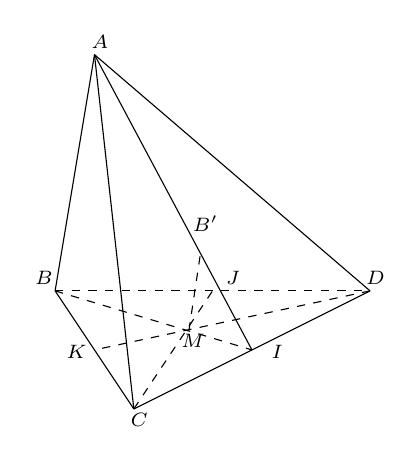
\begin{tikzpicture}[scale=0.5]
				\draw [dashed]  (2.,5.)-- (10.,5.);
				 \draw (2.,5.)-- (4.,2.);
				\draw (4.,2.)-- (10.,5.); 
				\draw  (3.,11.)-- (2.,5.);
				\draw  (3.,11.)-- (4.,2.);
				 \draw (3.,11.)-- (10.,5.);
				\draw  (3.,11.)-- (7.,3.5);
				\draw [dashed]  (2.,5.)-- (7,3.5);
				 \draw [dashed] (10.,5.)-- (3.,3.5);
				\draw  [dashed] (4.,2.)-- (6.,5.);
				\draw [dashed] (5.4,4)--  (5.7,6);
				\begin{scriptsize}
					\draw  (2.14,5.33) node[left] {$B$};
					\draw  (10.14,5.33) node {$D$};
					\draw  (4.14,2.1) node [below]{$C$};
					\draw (3.14,11.33)  node {$A$};
					 \draw (7.3,3.83) node [below right]{$I$};
					\draw  (3,3.81) node [below left]{$K$};
					\draw (6.14,5.33) node [right]{$J$}; 
					\draw  (5.5,4.1) node [below]{$M$};
					 \draw (5.82,6.31) node [above]{$B'$};
				\end{scriptsize}
			\end{tikzpicture}
		 }
	 }
\end{ex}

% nguồn: Ok_TraLoiNgan_Lop11_Lan1
\begin{ex}%[1H4V6-3]%[ma:58a72746]
	Cho tứ diện $ABCD$ và $M$ là điểm bất kì thuộc miền trong của tam giác $BCD$. Gọi $B'$, $C'$, $D'$ lần lượt là hình chiếu song song của $M$ theo các phương $AB$, $AC$, $AD$ lên các mặt  $(ACD)$, $(ABD)$, $(ABC)$. Tìm giá trị lớn nhất của $\dfrac{MB'}{AB}\cdot\dfrac{MC'}{AC}\cdot\dfrac{MD'}{AD}$ là $\dfrac{a}{b}$ với $a,b$ nguyên và $(a,b)=1$. Tính giá trị của $a+b$.
	\shortans{10} 
	 \loigiai{
	\immini{ 
		Trong tam giác  $ABI$ ta có $\dfrac{MB'}{AB}=\dfrac{MI}{BI}$.\\
		Tương tự ta cũng  có $\dfrac{MC'}{AC}=\dfrac{MJ}{CJ}$ và $\dfrac{MD'}{AD}=\dfrac{MK}{DK}$.\\
		Dễ thấy rằng $\dfrac{S_{MBD}}{S_{CBD}}=\dfrac{MJ}{CJ}$,  $\dfrac{S_{MCD}}{S_{BCD}}=\dfrac{MI}{BI}$, $\dfrac{S_{MBC}}{S_{DBC}}=\dfrac{MK}{DK}$.\\
		Cộng các đẳng thức với  nhau vế theo vế ta được
		$$\dfrac{MB'}{AB}+\dfrac{MC'}{AC}+\dfrac{MD'}{AD}=1.$$ 
		 }{
		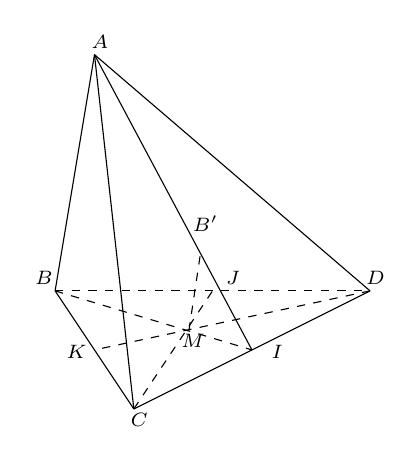
\begin{tikzpicture}[scale=0.5]
				 \draw [dashed] (2.,5.)-- (10.,5.);
				\draw  (2.,5.)-- (4.,2.);
				\draw  (4.,2.)-- (10.,5.);
				\draw  (3.,11.)-- (2.,5.);
				\draw (3.,11.)--  (4.,2.);
				\draw (3.,11.)--  (10.,5.);
				\draw (3.,11.)-- (7.,3.5); 
				\draw [dashed]  (2.,5.)-- (7,3.5);
				\draw  [dashed] (10.,5.)-- (3.,3.5);
				\draw  [dashed] (4.,2.)-- (6.,5.);
				\draw [dashed]  (5.4,4)-- (5.7,6);
				\begin{scriptsize}
					\draw  (2.14,5.33) node[left] {$B$};
					\draw (10.14,5.33)  node {$D$};
					\draw  (4.14,2.1) node [below]{$C$};
					\draw  (3.14,11.33) node {$A$};
					\draw (7.3,3.83) node  [below right]{$I$};
					\draw (3,3.81) node [below  left]{$K$};
					\draw (6.14,5.33)  node [right]{$J$};
					\draw (5.5,4.1) node [below]{$M$}; 
					\draw  (5.82,6.31) node [above]{$B'$};
				\end{scriptsize}
			\end{tikzpicture}
		 }
		Theo  bất đẳng thức AM-GM cho bộ ba số không âm ta có
		$$\dfrac{MB'}{AB}\cdot\dfrac{MC'}{AC}\cdot\dfrac{MD'}{AD}\leq  \left(\dfrac{\dfrac{MB'}{AB}+\dfrac{MC'}{AC}+\dfrac{MD'}{AD}}{3}\right)^3=\dfrac{1}{9}.$$
		Dấu bằng xảy ra khi $\dfrac{MB'}{AB}=\dfrac{MC'}{AC}=\dfrac{MD'}{AD}$ hay $\dfrac{MI}{BI}=\dfrac{MJ}{CJ}=\dfrac{MK}{DK}=\dfrac{1}{3}$, tức $M$  là trọng tâm tam giác $ABC$.
	} 
\end{ex}

% nguồn: Ok_TraLoiNgan_Lop11_Lan1
\begin{ex}%[1H4V6-3]%[ma:010fb13f]
	Cho hình chóp $S.ABCD$, đáy là hình thang ($AB\parallel CD$). Gọi $M$  là trung điểm của $SB$. Mặt phẳng qua $DM$, song song với $AB$ cắt đường thẳng $SC$ tại $Q$. Tính tỉ số $\dfrac{SC}{SQ}$.
	\shortans{1} 
	\loigiai{ 
	 \immini{
		Gọi $(\alpha)$  là mặt phẳng qua $DM$ và song song với $AB$. \\
		Vì $AB\parallel(\alpha)$ và $AB\subset(ABCD)$ nên giao tuyến của $(\alpha)$  và $(ABCD)$ là đường thẳng qua $D$ và song song với $AB$. Ta có $DC\parallel AB$ nên $DC$ chính là giao tuyến của $(\alpha)$ và $(ABCD)$. Do đó $(\alpha)$ cắt $SC$ tại $C$, tức là $Q$ trùng với $C$. Vì vậy $\dfrac{SC}{SQ}=1$. }{
		\begin{tikzpicture}[scale=1,font=\footnotesize,line join=round,line cap=round,>=stealth]
				 \def\bc{4}
				 \def\ba{2}
				\def\h{4} 
				\def\gocB{30} 
				\coordinate[label=below  left:$B$] (B) at (0,0);
				\coordinate[label=above left:$A$] (A) at  (\gocB:\ba);
				\coordinate[label=below:$C$] (C) at (\bc,0); 
				\coordinate[label=right:$D$] (D) at  ($.8*(A)-.8*(B)+(C)$);
				\coordinate[label=above:$S$] (S) at  ($(A)+(0:.5)+(90:\h)$);
				\coordinate[label=left:$N$] (N)  at ($(A)!.5!(S)$);
				\coordinate[label=left:$M$] (M) at ($(B)!.5!(S)$); 
				\draw (B)--(C)--(D)--(S)--cycle (S)--(C)--(M); 
				\draw[dashed]  (A)--(D)--(M)--(N)--(D)
					 (S)--(A)--(B);
				\foreach \diem in {A,B,C,D,S,M,N}  \fill (\diem) circle (1pt);
			\end{tikzpicture}
		} 
	 }
\end{ex}

% nguồn: Ok_TraLoiNgan_Lop11_Lan1
\begin{ex}%[1H4V6-3]%[ma:87016dbf]
	Cho tứ diện đều $ABCD$ có  cạnh bằng $a$. Gọi $M,N$ lần lượt là trọng tâm của $\Delta ABC$ và $\Delta ABD$. Diện tích thiết diện của tứ diện khi cắt bởi mặt phẳng $(BMN)$ là $\dfrac{a^2\sqrt{a}}{b}$. Khi đó $a+b$ bằng
	\shortans{27} 
	\loigiai{ 
		\begin{center}
			\begin{tikzpicture}[scale=1.3]
					\coordinate (A) at  (2,3); \coordinate (B) at (0,0);
					\coordinate (C) at  (1.5,-2); \coordinate (D) at (4,0);
					\coordinate (E)  at ($(A)!.5!(C)$);
					\coordinate (F) at ($(A)!.5!(D)$); 
					\draw  (A) node[above]{$A$}--(B) node[left]{$B$}--(C) node[below]{$C$}--(D) node[right]{$D$}--cycle;
					 \draw (A)--(C);
					\draw (B)--  (E) node[below right]{$E$} -- (F) node[right]{$F$};
					\draw  [dashed] (B)--(F); \draw [dashed] (B)--(D);
					\coordinate  (M) at ($(B)!2/3!(E)$);
					 \coordinate (N) at ($(B)!2/3!(F)$);
					\draw[fill] (M) circle  (1pt) node[below]{$M$};
					 \draw[fill] (N) circle (1pt) node[above]{$N$};
				\end{tikzpicture}
		\end{center}
		Trong $(ABD)$, $BN$ cắt $AD$ tại $F$. Trong $(ABC),  BM$ cắt $AC$ tại $E$.\\
		Do $M,N$ lần lượt là trọng tâm của $\Delta ABD$ nên $E,F$ lần lượt là trung điểm của  $AC,AD$.\\
		Tứ  diện $ABCD$ có cạnh bằng $a$ nên $BE=BF=\dfrac{a\sqrt{3}}{2}$.\\
		Thiết diện là tam giác cân $BEF$ tại  $B$, có cạnh đáy $EF=\dfrac{a}{2}$.\\
		Diện tích $\Delta BEF$  là $S_{BEF}=\dfrac{1}{2}.\dfrac{a}{2}.\sqrt{\left(\dfrac{a\sqrt{3}}{2}\right)^2-\left(\dfrac{a}{4}\right)^2}=\dfrac{a^2\sqrt{11}}{16}$ (đvdt).\\
		Suy  ra $a+b=27$.
	 }
\end{ex}

% nguồn: Ok_TraLoiNgan_Lop11_Lan2
\begin{ex}%[1H4V6-3]%[ma:841e2d30]
	Cho hình hộp chữ nhật $ABCD.A'B'C'D'$. Xác định các điểm $M$, $N$ tương ứng trên các đoạn $AC'$, $B'D'$ sao cho $MN$ song song với $BA'$ và  tính tỉ số $\dfrac{MA}{MC'}$.
	 \shortans{2}
	\loigiai{ 
		\begin{center}
			\begin{tikzpicture}[scale=1,font=\footnotesize,line join=round,line cap=round,>=stealth]
					\path (0,3)  coordinate (h)
						(0,0) coordinate (B)++(2.5,0) coordinate (A)++(1,0.8)  coordinate (D)
						($(B)+(D)-(A)$) coordinate  (C);
					\foreach \p in {A,B,C,D}\path  ($(\p)+(h)$) coordinate (\p');
					\path ($2*(A')-(B')$) coordinate (K) 
						 (intersection of B'--D' and K--C') coordinate (N)
						($(C')!1/3!(A)$) coordinate (M) 
						(intersection of D--D' and  A--K) coordinate (d)
						(intersection of D--D'  and C'--K) coordinate (d');
					\draw (C')--(B')--(B)--(A)--(D)--(d) 
						 (d')--(D')--(C')
						 (B')--(A')--(D')--(B')
						(C')--(K)--(A)--(A')--(B) 
						 (K)--(A');
					\draw[dashed]  (B)--(C)--(D)
						(C)--(C')--(A) 
						(M)--(N) 
						(d)--(d'); 
					\foreach \p/\g in {C/45,B/240,A/-60,D/0,C'/90,B'/180,A'/-45,D'/45,K/30,N/-90,M/-120} \fill[black] (\p) circle (1pt)+(\g:0.3) node{$\p$}; 
				\end{tikzpicture}
		\end{center}
		Xét phép chiếu song  song lên mặt phẳng $\left(A'B'C'D'\right)$ theo phương $BA'$, ta có
		$N$ là hình chiếu của $M$ hay $N$ là giao điểm của $B'D'$ với hình chiếu của  $AC'$ qua phép chiếu này.\\
		 Do đó ta xác định được $M,N$ như sau
		\begin{itemize}
			\item Trên tia $B'A'$, lấy điểm $K$ sao cho  $A'K=B'A'$ thì $ABA'K$ là hình bình hành nên $AK\parallel BA'$, suy ra $K$ là hình chiếu của $A$ qua phép chiếu song song.
			\item Gọi $N=B'D'\parallel KC'$. Đường thẳng qua $N$ và song song với $AK$ cắt  $AC'$ tại $M$.
		\end{itemize}
		Từ đó  ta xác định được điểm $M,N$ cần tìm.\\
	Theo  định lý Thales, ta có $\dfrac{MA}{MC'}=\dfrac{NK}{NC'}=\dfrac{KB'}{C'D'}=2$.}
\end{ex}
